
%使用XeLaTeX编译
%版权所有,翻版必究
%本文件由程序自动生成,任何修改将被覆盖
%2019 年 01 月 23 日




\FloatBarrier
\section{
HueSaturation
}\label{c000015s000008}


%begin图片
\begin{figure}[htb] %浮动体 here and top ...
%there must use marginnote ...
\marginnote{\setlength\fboxsep{2pt}\fbox{\footnotesize{\kaishu\figurename\,}\footnotesize{\ref{p000024}}}}\centering %中心对齐
\setlength\fboxsep{0pt}\fcolorbox[rgb]{0,0,0}{0,0,0}{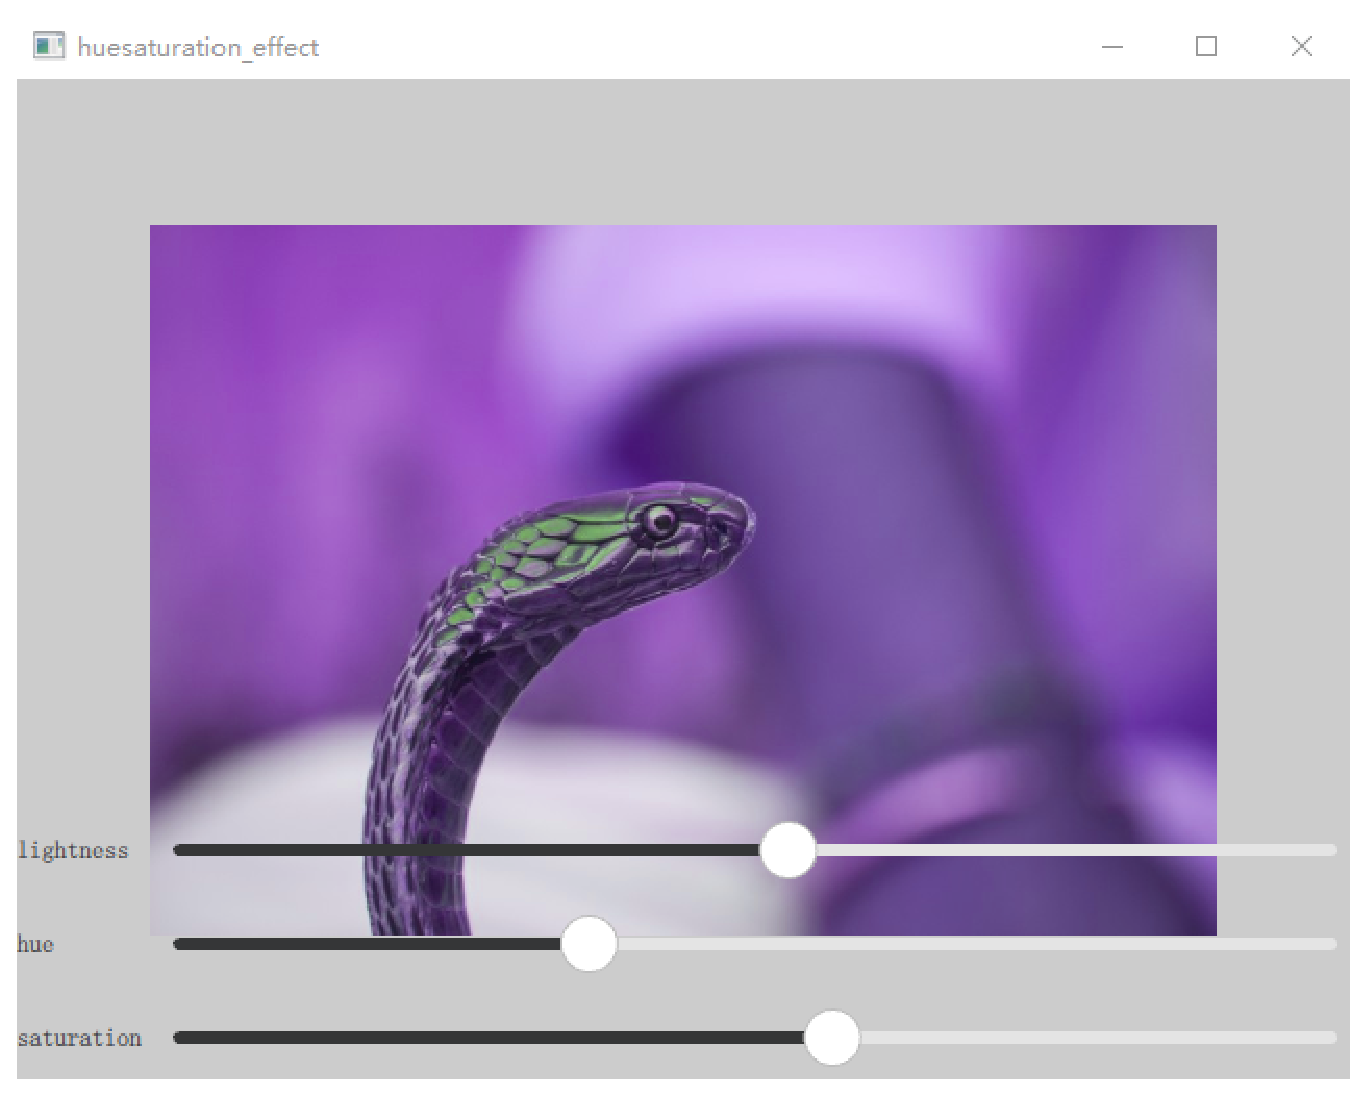
\includegraphics[width=0.95\textwidth]{the_book_image/p000024.eps}} %图片路径
\caption{HueSaturation} %标题
\label{p000024} %索引
\end{figure}
%end图片


%\begin{spacing}{1.0}
\refstepcounter{filesourcenumber}\label{f000058}    %增加源代码编号
\FloatBarrier                                  %强制完成浮动体布局
\begin{thebookfilesourceone}[escapeinside={(*@}{@*)},
caption=GoodLuck,
title=\filesourcenumbernameone \thefilesourcenumber
]
/*huesaturation_effect/main.qml*/
import QtQuick 2.9
import QtGraphicalEffects 1.12

Rectangle {
    id : idRoot
    width: 640;
    height: 480;
    color: Qt.rgba(0.8,0.8,0.8,1);

    Image{
        width: parent.width * 0.8;
        height: parent.height * 0.8;
        anchors.centerIn: parent
        source: "image"
        visible: false
        fillMode: Image.PreserveAspectFit
        id : idImage
    }

    HueSaturation{
        anchors.fill: idImage
        source: idImage
        hue : thisControl.hueItem.value
        lightness: thisControl.lightnessItem.value
        saturation: thisControl.saturationItem.value
    }

    HuesaturationControl{
        id : thisControl
    }

}(*@\marginpar[\hfill\setlength\fboxsep{2pt}\fbox{\footnotesize{\kaishu\parbox{1em}{\setlength{\baselineskip}{2pt}\filesourcenumbernameone}}\footnotesize{\thefilesourcenumber}}]{\setlength\fboxsep{2pt}\fbox{\footnotesize{\kaishu\parbox{1em}{\setlength{\baselineskip}{2pt}\filesourcenumbernameone}}\footnotesize{\thefilesourcenumber}}}@*)\end{thebookfilesourceone}          %抄录环境
\addtocounter{lstlisting}{-1}   %sub lstlisting counter ...
%\end{spacing}


未完待续






%使用XeLaTeX编译
%版权所有,翻版必究
%本文件由程序自动生成,任何修改将被覆盖
%2019 年 01 月 23 日



